% Hall-current sampling: 4 ADC triggers per PWM period from the HRTIM, 80-sample box average per control tick
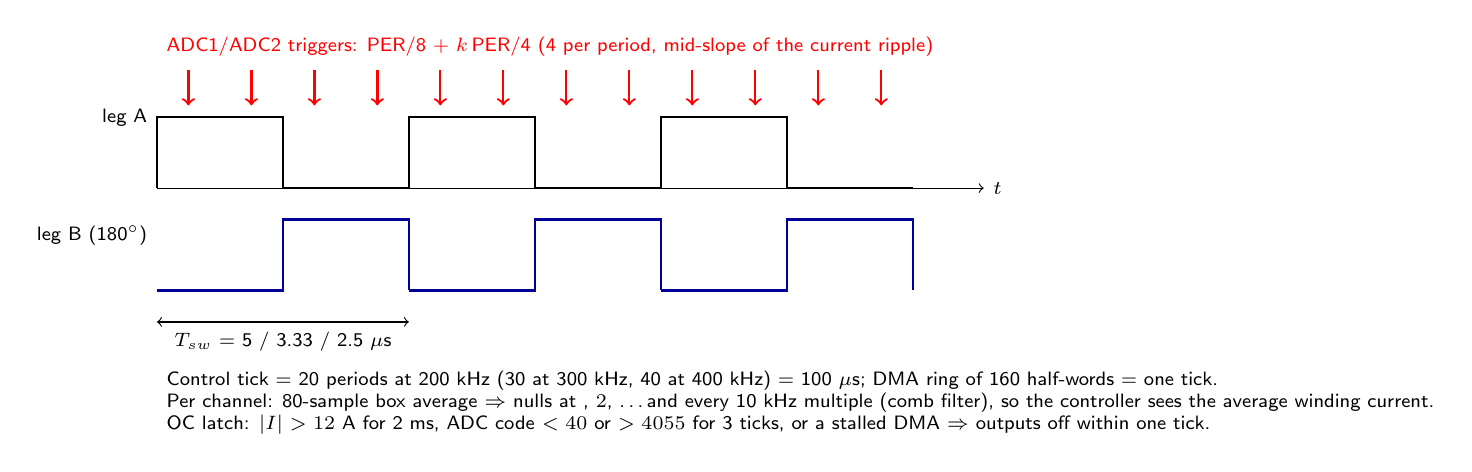
\begin{tikzpicture}[x=1cm,y=1cm,font=\sffamily\scriptsize]
  % PWM period axis
  \draw[->] (0,0) -- (10.5,0) node[right]{$t$};
  \foreach \i in {0,1,2}{
    \draw[thick] (\i*3.2,0) -- (\i*3.2,0.9) -- (\i*3.2+1.6,0.9) -- (\i*3.2+1.6,0) -- (\i*3.2+3.2,0);
  }
  \node[left] at (0,0.9) {leg A};
  \foreach \i in {0,1,2}{
    \draw[thick,blue!60!black] (\i*3.2,-1.3) -- (\i*3.2+1.6,-1.3) -- (\i*3.2+1.6,-0.4) -- (\i*3.2+3.2,-0.4) -- (\i*3.2+3.2,-1.3);
  }
  \node[left] at (0,-0.6) {leg B (180$^\circ$)};
  % triggers at PER/8 + k PER/4
  \foreach \i in {0,1,2}{\foreach \k in {0,1,2,3}{
    \draw[red,thick,->] (\i*3.2+0.4+\k*0.8,1.5) -- (\i*3.2+0.4+\k*0.8,1.05);
  }}
  \node[red,anchor=south west] at (0,1.55) {ADC1/ADC2 triggers: PER/8 + $k$\,PER/4 (4 per period, mid-slope of the current ripple)};
  \draw[<->] (0,-1.7) -- node[below]{$T_{sw}$ = 5 / 3.33 / 2.5 $\mu$s} (3.2,-1.7);
  \node[align=left,anchor=north west] at (0,-2.2) {Control tick = 20 periods at 200 kHz (30 at 300 kHz, 40 at 400 kHz) = 100 $\mu$s; DMA ring of 160 half-words = one tick.\\
  Per channel: 80-sample box average $\Rightarrow$ nulls at $\fsw$, $2\fsw$, \ldots and every 10 kHz multiple (comb filter), so the controller sees the average winding current.\\
  OC latch: $|I| > 12$ A for 2 ms, ADC code $<40$ or $>4055$ for 3 ticks, or a stalled DMA $\Rightarrow$ outputs off within one tick.};
\end{tikzpicture}
